\documentclass{article}[a4paper]
\usepackage[a4paper, total={7in, 10in}]{geometry}
\usepackage[T1]{fontenc}
\usepackage{charter}
\usepackage{xcolor}
\usepackage{graphicx}
\usepackage{float}
\usepackage{listings}
\usepackage{amsmath}
\usepackage{amssymb}
\usepackage{enumitem}
\usepackage{tabularray}

\lstset{
  language=Python,
  basicstyle=\ttfamily,
  keywordstyle=\color{blue},
  commentstyle=\color{gray},
  stringstyle=\color{red},
  showstringspaces=false,
  columns=fullflexible,
  breaklines=true
}

\title{
	\huge{\textbf{
		Assignment 01
	}}\\
	\Large{
		Intensity Transformations and Neighborhood Filtering
	}\\
	\phantom{}\\
	\large{
		submitted for
	}\\
	\LARGE{
		\textbf{EN3160 - Image Processing and Machine Vision}
	}\\
	\large{
		Department of Electronic and Telecommunication Engineering
	}
	\\
	\large{University of Moratuwa}
}

\author{
	\textbf{Udugamasooriya P. H. J.}\\
	220658U\\
}

\date{12 August 2025}

\allowdisplaybreaks

\begin{document}

\maketitle

\begin{enumerate}
	\item The given transformation is exactly the identity transformation except in the interval from $50$ to $150$, where, if
	the value of a pixel in the original image is denoted by $x$, and its image under the transformation is denoted by $y$, we have \[
		\dfrac{y - 100}{x - 50} = \dfrac{255 - 100}{150 - 50} = 1.55,
	\] which gives \[
		y = 1.55x + 22.5.
	\] This is implemented in the code by first constructing a vector \lstinline|T| representing the identity transformation and then using 
	\lstinline|T[50:151] = 1.55 * T[50:151] + 22.5| to alter only the required portion of it as desrcibed above.

	The output is as follows;
	\begin{figure}[H]
		\centering
		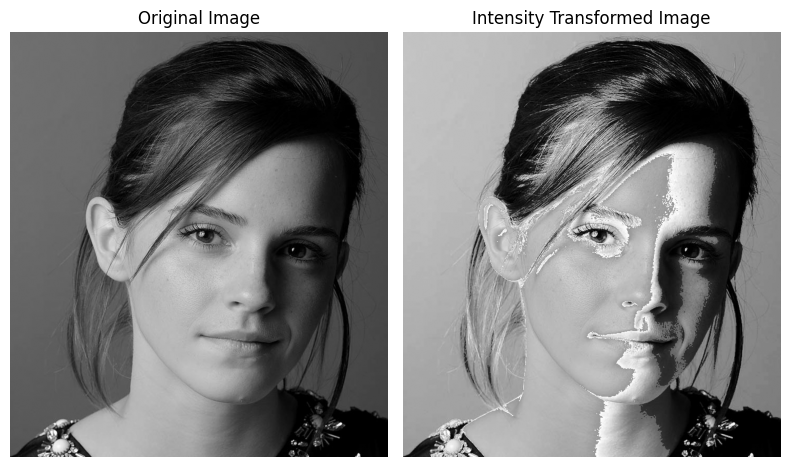
\includegraphics[width=0.7\linewidth]{images/q1.png}
		\caption{Question 1}
	\end{figure}

	\item An eyedropper tool was used to inspect the values of a few representative pixels from the graymatter and whitematter areas and
	it was observed that pixel intensities less than about $175$ correspond to graymatter. To highlight these pixels, we implement the transformation
	given by \[
		\begin{cases}
			x \texttt{ // } 6, & x \leq 175,		\\
			x,		& \text{otherwise},
		\end{cases}
	\] where \texttt{//} denotes the integer-division operation (integer quotient upon division); i.e., we proportionally suppress the 
	intensities of the pixels darker than $175$, and leave the rest unaffected.
	
	A vector denoting this transformation is easily created
	by first creating \lstinline|T| as described above and then executing \lstinline|T[0:175] = T[0:175] // 6|.

	The results are as follows;
	\begin{figure}[H]
		\centering
		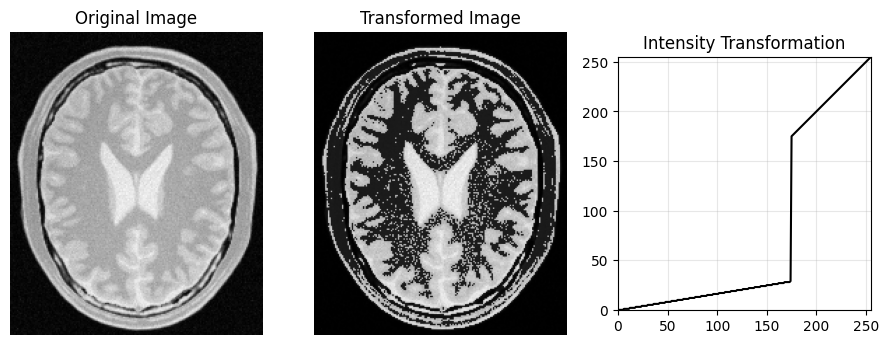
\includegraphics[width=\linewidth]{images/q2.png}
		\caption{Question 2}
	\end{figure}

	\item We open the image, \lstinline|cv2.cvtColor| it from BGR to the LAB color scheme, and extract the L-channel. We then apply the
	gamma transformation specified by \[
		T(x) = 255 \cdot \left(\dfrac{x}{255}\right) ^ \gamma
	\] to the L-channel. The most aesthetically pleasing result was obtained by setting $\gamma = 0.5$. The results are given below.

	\begin{figure}[H]
		\centering
		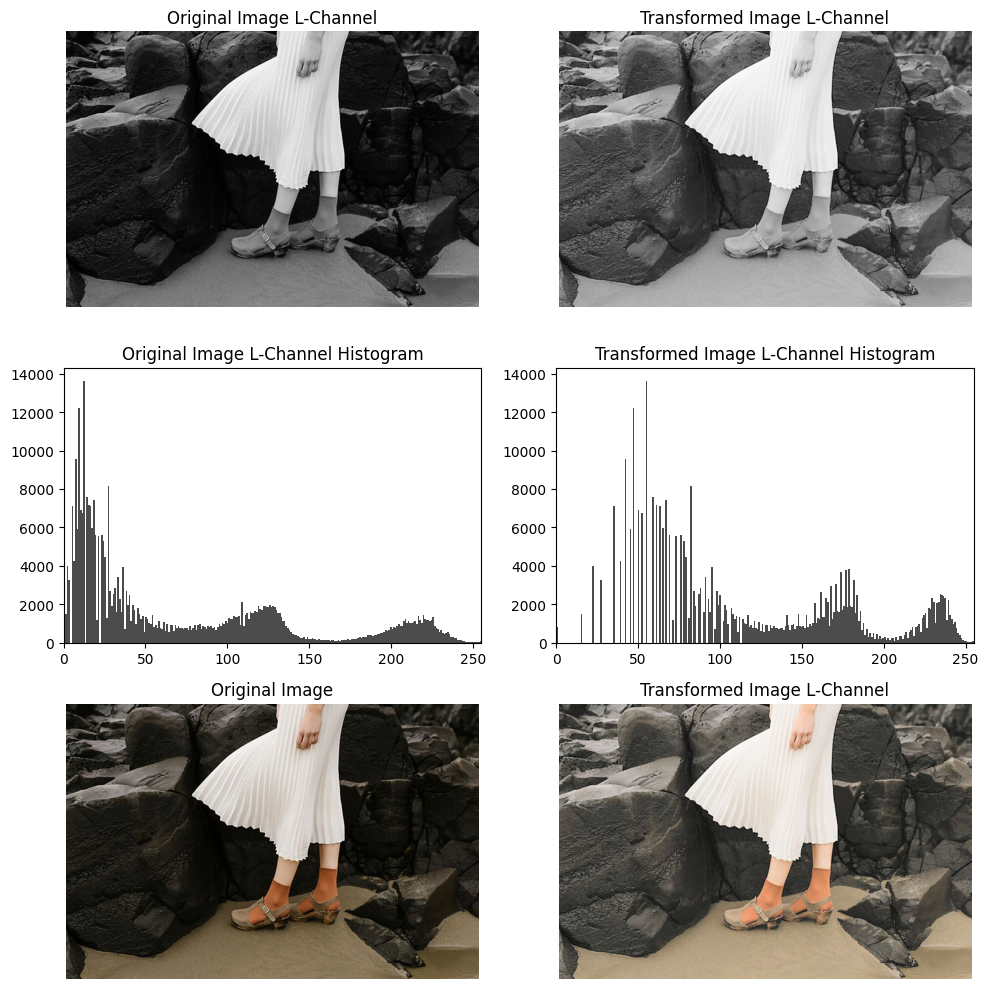
\includegraphics[width=0.9\linewidth]{images/q3.png}
		\caption{Question 3}
	\end{figure}
	
	\item The lines
	\begin{lstlisting}[language=Python]
a = 0.65
sigma = 70

T = np.arange(256, dtype=np.float32)
T = np.minimum(np.ones(256) * 255, T + a * 128 * np.exp(-((T - 128) ** 2) / (2 * sigma ** 2)))
	\end{lstlisting}
	implement the intensity transformation. We provide one vector where all entries are $255$. and another vector populated with entries
	computed according the expression given, and use \lstinline|np.minimum| to pick the smaller of the two. The most aesthetically
	pleasing result was obtained by setting $a = 0.65$. The results are as follows;

	\begin{figure}[H]
		\centering
		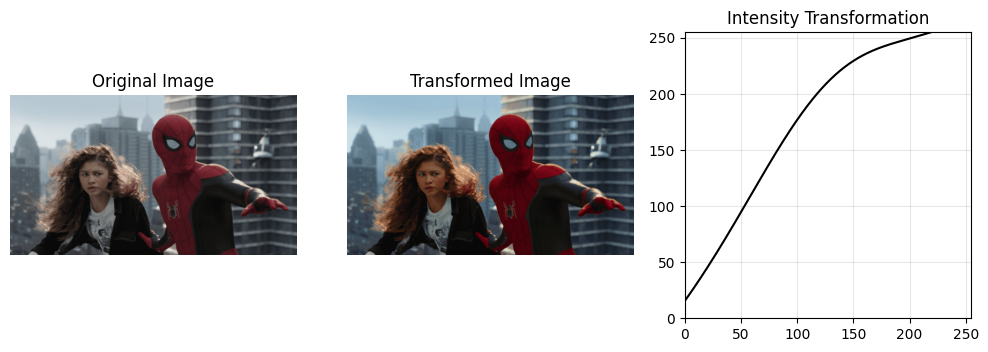
\includegraphics[width=0.9\linewidth]{images/q4.png}
		\caption{Question 4}
	\end{figure}

	\item It is required to apply a transformation to the pixels such that the distribution of the pixels after transformation is (at least
	nearly) uniform over the range $0$ to $255$.
	
	Let $X$ be a random variable denoting the value of a pixel randomly chosen from the image.
	The normalized histogram of the image may be treated as the p.m.f. of $X$. We require an injective transformation $T:[0, 255] \to [0, 255]$,
	such that the p.m.f. of the random variable $Y=T(X)$ is uniform, i.e., equal to $\dfrac{1}{255}$ over all possible values of $Y$.

	To proceed, we will also assume that the $T$ we seek is surjective, and hence bijective. Let $y \in [0, 255]$, i.e., let 
	$y$ be one of the values that $Y$ might assume. Because we require the p.m.f. of $Y$ to uniform, we must have
	\begin{align*}
		\text{Pr}\left( Y \leq y \right) &= \dfrac{y}{255} \\
		\text{Pr}\left( T(X) \leq y \right) &= \dfrac{y}{255} \\
		\text{Pr}\left( X \leq T^{-1}(y) \right) &= \dfrac{y}{255}.
	\end{align*}

	The last equation above gives the probability of $X$ being less than the value $T^{-1}(y)$. Let $x$ be one of the
	possible values that $X$ may take, and suppose that $y$ is such that $T^{-1}(y) = x$, or equivalently, $y = T(x)$. Then, the
	expressions $\text{Pr}\left( X \leq x \right)$ and $\text{Pr}\left( X \leq T^{-1}(y) \right)$
	both denote the same quantity, so we can write \[
		\text{Pr}\left( X \leq x \right) = \dfrac{T(x)}{255}.
	\]
	
	But, the c.d.f. of $X$ is just the running sum of its p.m.f. which is known. Hence, denoting the number of pixels having intensity
	level $i$ by $n_i$, we have \[
		\dfrac{T(x)}{255} = \text{Pr}\left( X \leq x \right) = \dfrac{1}{LM} \sum_{j = 1}^x n_j,
	\] where $L$ and $M$ give the dimensions of the image in pixels.
	
	This gives the transformation we seek; \[
		T(x) = \dfrac{255}{LM} \sum_{j = 1}^x n_j.
	\] This is also the transformation implemented in the following lines of code;
	\begin{lstlisting}[language=Python]
def equalize_histogram(img):
    pixel_values, counts = np.unique(img, return_counts=True)
    cumulative_counts = np.cumsum(counts)

    T = np.arange(256, dtype=np.uint8)

	for i in range(len(pixel_values)):
        pixel_value = pixel_values[i]
        T[pixel_value] = np.round((cumulative_counts[i] / cumulative_counts[-1]) * 255)

    return T[img]
	\end{lstlisting}
	We first extract the distinct pixel values present in the image, and use \lstinline|np.cumsum| to form a running sum of the number
	of pixels of each intensity level. The transformation is constructed such that it leaves pixels that are not present in the image
	unchanged (it should not matter what they are mapped to, as they are simply not present in the image), but those present are mapped
	to the intensity level computed as described above in terms of the cumulative sum.

	The result of the entire process is shown below.

	\begin{figure}[H]
		\centering
		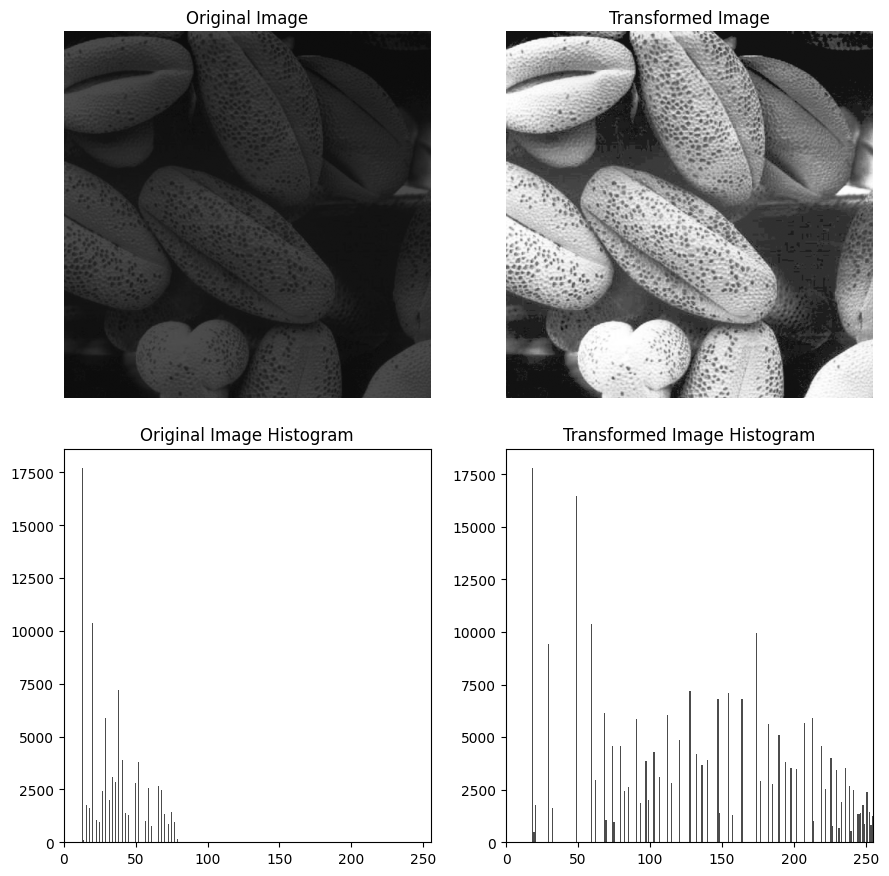
\includegraphics[width=0.8\linewidth]{images/q5.png}
		\caption{Question 5}
	\end{figure}

	\item The background of the given image is predominantly composed of light colors. Hence, we expect the pixel values corresponding
	to the background in the S channel of the image in its HSV representation to be mostly small values. Hence, we apply a threshold in
	the S channel using \lstinline|cv2.threshold|. By trial and error, the suitable value for thresholding was found to be $11$.

	Thresholding yields a binary image, i.e., the foreground mask, where the foreground pixels are white and background pixels are black.
	We then perform \lstinline|cv2.bitwise_and| of the mask with the S and V channels to extract the foreground from each channel. Further,
	\lstinline|cv2.bitwise_not| of the mask yields the background mask. We perform \lstinline|cv2.bitwise_and| of each channel with the 
	background mask too to obtain the background from each channel.

	We then implement the \lstinline|equalize_histogram| function, which is based on the formulas given in the slides, and is very
	similar to the function implemented in the previous question, except for some slight modifications in the line
	\begin{lstlisting}[language=Python]
T[pixel_value] = np.round(((cumulative_counts[i] - cumulative_counts[0]) / (cumulative_counts[-1] - cumulative_counts[0]) ) * 255),
	\end{lstlisting}
	made to ignore the zero-valued pixels. This is done because the zero-valued pixels correspond to pixels in the background, and the
	probability that a pixel of a certain value be found in the foreground must be found without considering pixels in the background.

	We use this function to equalize the histograms of the foregrounds in the S and V channels, but leave the H channel unchanged, as it
	contains information about the color of each pixel which must be preserved. Finally, we combine the histogram-equalized foregrounds
	from the S and V channels with the H channel of the original image, and construct the final image.

	The results are as follows.

	\begin{figure}[H]
		\centering
		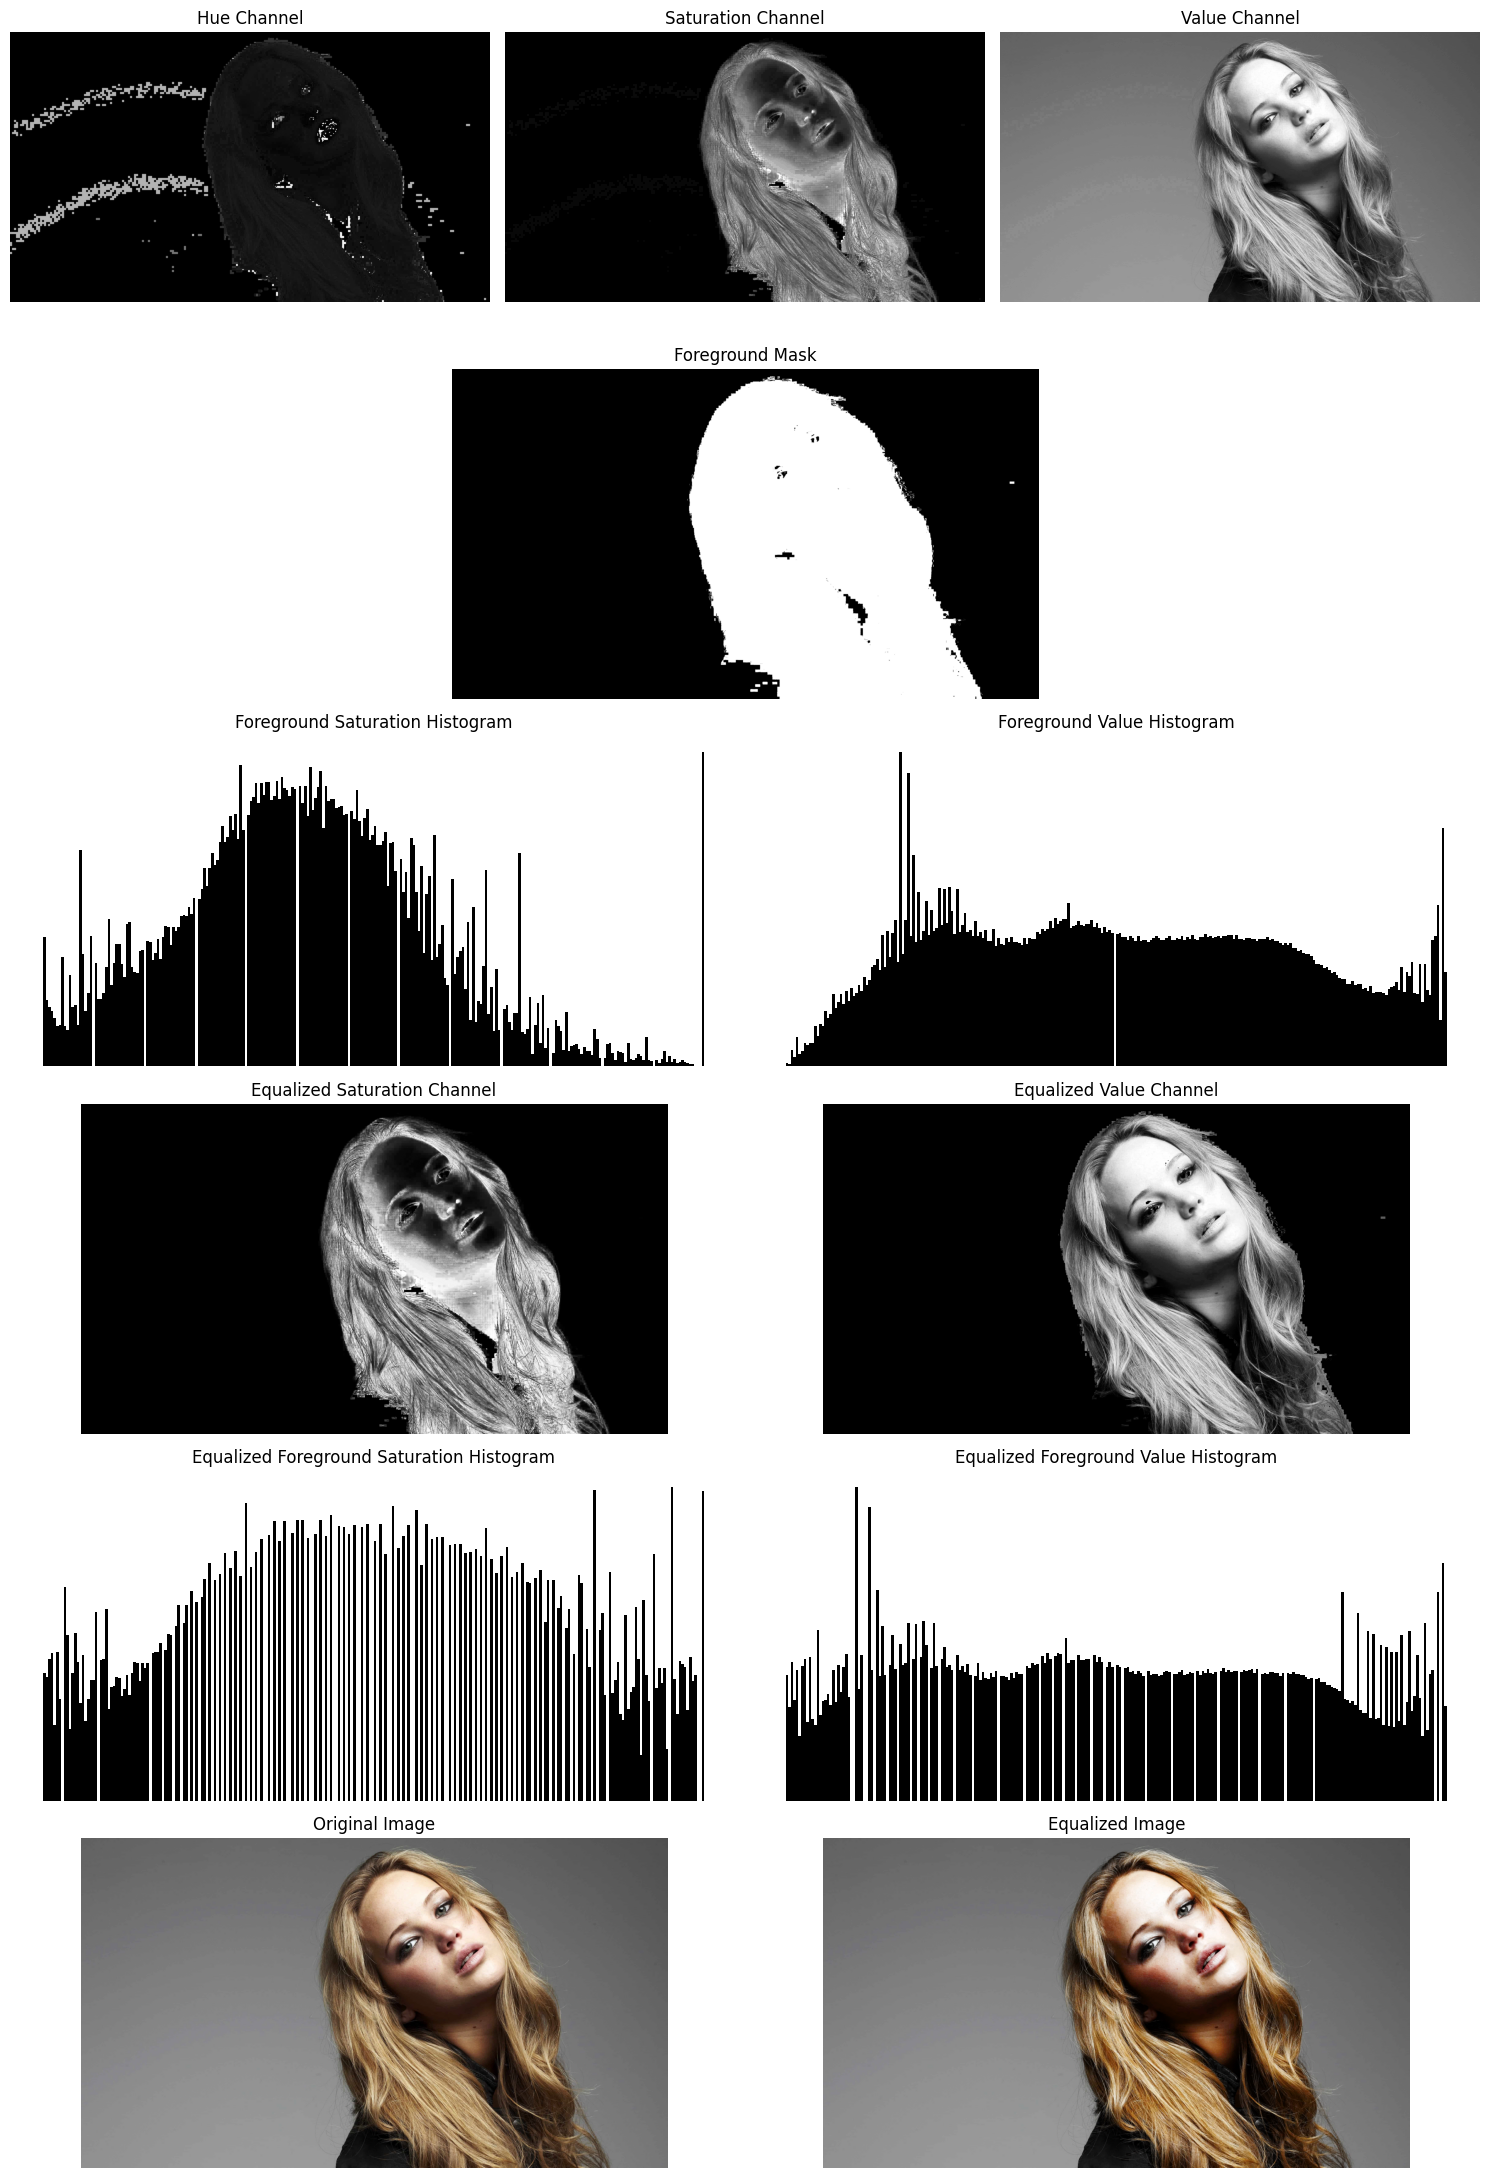
\includegraphics[width=0.8\linewidth]{images/q6.png}
		\caption{Question 6}
	\end{figure}

	\item 
	
\end{enumerate}

\end{document}